% !Mode:: "TeX:UTF-8"
\chapter{Cameras and Images}
\label{cpt:5}
\begin{mdframed}  
	\textbf{Goal of This Chapter}
	\begin{enumerate}[labelindent=0em,leftmargin=1.5em]
		\item Understand the pin-hole camera model, intrinsics, extrinsics and distortion. 
		\item Understand how to project a spatial point into image planes. 
		\item Understand how to cope with the OpenCV images. 
		\item Understand the basic calibration methods. 
	\end{enumerate}
\end{mdframed} 

In the previous two lectures, we introduced the problem that how to express and optimize the robot's 6 DoF pose, and partially explained the meaning of the variables and the equations of motion and observation in SLAM. In this chapter we will discuss ``How robots observe the outside world'', which is part of the observation equation. In the camera-based visual SLAM, the observation mainly refers to the process of \textbf{image projection}.

We can see a lot of photos in real life. In a computer, a photo consists of millions of pixels, each of which records the information about color or brightness. We will see a bundle of light reflected or emitted by an object in the three-dimensional world pass through the camera's optical center and is projected onto the imaging plane of the camera. After the camera's light sensor receives the light, it produces a measurement and we get the pixels, which form the photo we see. Can this process be described by mathematical equations? This lecture will first discuss the camera model, explain how the projection relationship is described, and what is the internal parameters in this projection process. At the same time, we are also going to give a brief introduction to the stereo and RGB-D cameras. Then, we introduce the basic operations of 2D images in OpenCV. Finally, an experiment of point cloud stitching is demonstrated to show the meaning of intrinsics and extrinsics parameters.

\newpage
\section{Pin-hole Camera Models}
The process of projecting a 3D point (in meters) to a 2D image plane (in pixels) can be described by a geometric model. Actually there are several models to describe this, the simplest of which is called the \textbf{pinhole model}. We will start from this pin-hole projection. At the same time, due to the presence of the lens on the camera lens, \textbf{distortion} is generated during the projection. Therefore, we are going to use the pin-hold model plus with a distortion model to describe the entire projection process.

\subsection{pinhole camera model}
Most of us have seen the candle projection experiment in the physics class of high school: a lit candle is placed in front of a dark box, and the light of the candle is projected through a small hole in the dark box on the rear plane of the black box. Then an inverted candle image is formed on this plane. In this process, the small hole is able to project a candle in a three-dimensional world onto a two-dimensional imaging plane. For the same reason, we can use this simple model to explain the imaging process of the camera, as shown in \autoref{fig:cameraModel}.

\begin{figure}[!ht]
	\centering
	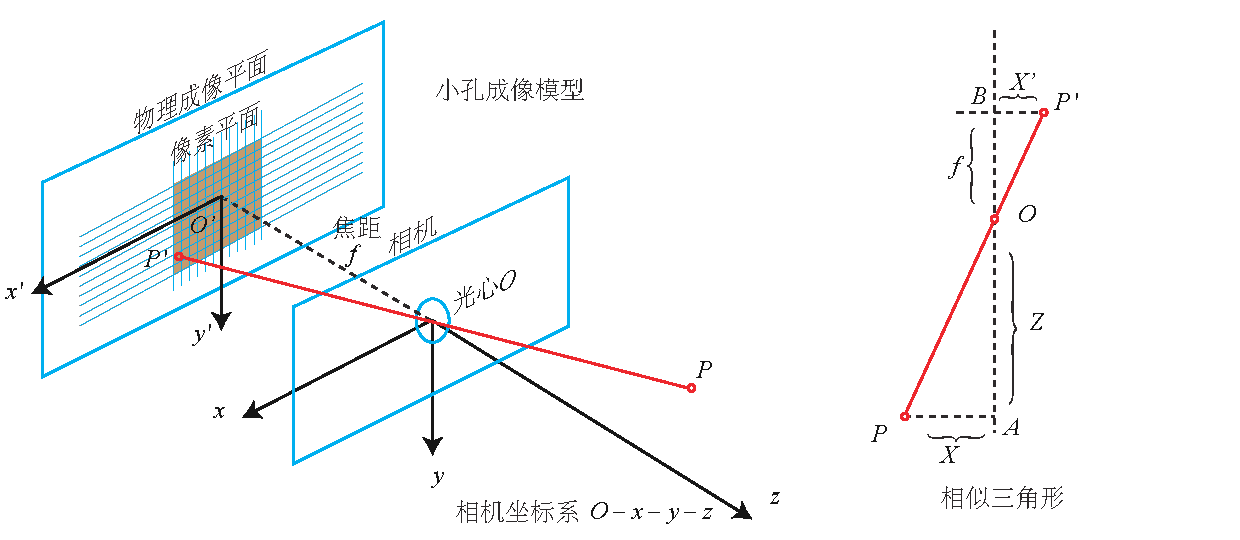
\includegraphics[width=.95\textwidth]{cameraModel/cameraModel.pdf}
	\caption{Pinhole camera model. }
	\label{fig:cameraModel}
\end{figure}

Let's take a look at the simple geometry in this model. Let $O-x-y-z$ be the camera coordinate system. Commonly we put the $z$ axis to the front of the camera, $x$ to the right, and $y$ to the down (so in this figure we should stand on the left side to see the right side). $O$ is the camera's \textbf{Optical Center}, which is also the ``hole'' in the pinhole model. The 3D point $P$, after being projected through the hole $O$, falls on the physical imaging plane $O'-x'-y'$, and produce the image point $P'$. Let the coordinates of $P$ be $[X,Y,Z]^\mathrm{T}$, $P'$ is $[X',Y',Z']^\mathrm{T}$, and set the physical distance from the imaging plane to camera plane is $f$ (focal length). Then, according to the similarity of the triangles, there are:
\begin{equation}
\frac{Z}{f} = -\frac{X}{{X'}} =-\frac{Y}{{Y'}}.
\end{equation}
The negative sign indicates that the image is inverted. However, the image obtained by the actual camera is not an inverted image (otherwise the usage of the camera would be very inconvenient). In order to make the model more realistic, we can equivalently place the imaging plane symmetrically in front of the camera, along with the 3D space points on the same side of the camera coordinate system, as shown by \autoref{fig:planes}. This can remove the negative sign in the formula to make the formula more compact:

\begin{equation}
\frac{Z}{f} = \frac{X}{{X'}} =\frac{Y}{{Y'}}.
\end{equation}

\begin{figure}[!htp]
	\centering
	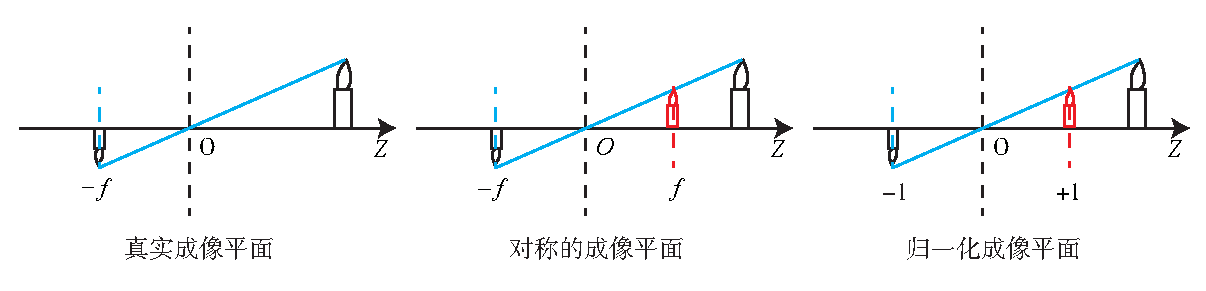
\includegraphics[width=1.0\textwidth]{cameraModel/planes.pdf}
	\caption{The real, symmetric and normalized image plane.}
	\label{fig:planes}
\end{figure}

Put $X', Y'$ to the left side:
\begin{equation}\label{eq:P2Pprime}
\begin{array}{l}
X' = f\frac{X}{Z}\\
Y' = f\frac{Y}{Z}
\end{array}.
\end{equation}
